\documentclass[11pt]{article}
\usepackage{amsmath, amsthm, amssymb}
\usepackage{array,mathtools}
\usepackage[textwidth=8in,textheight=9in]{geometry}
% \newcommand\showdiv[1]{\overline{\smash{\hstretch{.5}{)}\mkern-3.2mu\hstretch{.5}{)}}#1}}
% \newcommand\ph[1]{\textcolor{white}{#1}}
% \newcommand*{\carry}[1][1]{\overset{#1}}
% \newcolumntype{B}[1]{r*{#1}{@{\,}r}}
\usepackage{listings}
\usepackage{courier}
\setlength{\oddsidemargin}{-1cm}
\setlength{\evensidemargin}{0cm}
\setlength{\textwidth}{500pt}

\usepackage{color}
\usepackage{wrapfig}
\usepackge(multirow)

\usepackage{listings}
\usepackage{color}

\definecolor{mygreen}{rgb}{0,0.6,0}
\definecolor{mygray}{rgb}{0.5,0.5,0.5}
\definecolor{mymauve}{rgb}{0.58,0,0.82}

\usepackage{courier}

\lstset{basicstyle=\footnotesize\ttfamily,breaklines=true}
\lstset{framextopmargin=50pt,frame=bottomline}


\title{Individual Project}
\author{Luka Milic: lm1015}

\begin{document}
\maketitle
\section{Introduction}
% Most data is unlabeled [http://arxiv.org/abs/1603.08262]
The aim of the project is to implement a neural network which can take both labelled and unlablled face images.
This is relevant to the field of pattern recogintion because real life data is often unlabeled. Infact most learning is unsupervised.
\section{Theory}
Neural networks and stuff
\section{Model}
\begin{figure}
  \begin{center}
    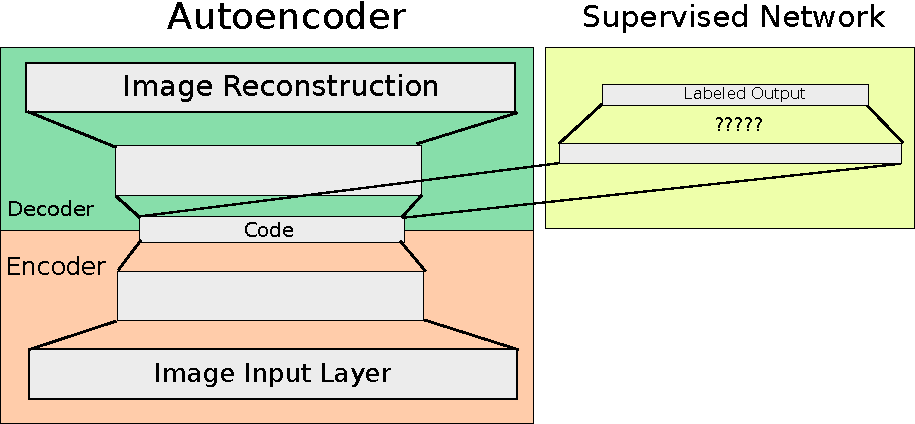
\includegraphics[width=0.5\textwidth]{illustrations/network_01.pdf}
  \end{center}
  \caption{Basic structure of the network}
\end{figure}
really nice models
The idea is to manually set the gradient to zero on unlabled modes. To create a unified cost function so the network can be trained at once.
\section{Data}
DISFA
\section{Evaluation Method}
Need to use some metrics.
\section{Results}
\section{Progress}
\subsection{First target}
implement the basic network with mnist data, compare various cost functions

\begin{tabular}{c | c c | c | l}
& Sprint && Time & Topic \\\hline
\multirow{9}{*}{\rotatebox[origin=c]{90}{Alex Carver}}
    & 11-Jan & 24-Jan & 23 & Background Research \\
    & 25-Jan & 07-Feb & 37 & ESTMD, Report Writing \\
    & 08-Feb & 21-Feb & 46 & ESTMD\\
    & 22-Feb & 06-Mar & 44 & DragonflyBrain\\
    & 07-Mar & 20-Mar & 24 & DragonflyBrain, Report Writing\\
    & 21-Mar & 03-Apr & 21 & Testing\\
    & 04-Apr & 17-Apr & 48 & Environment\\
    & 18-Apr & 01-May & 25 & Environment, RL\\
    & 02-May & 15-May & 82 & Environment, RL, Report Writing\\
    \hline
\end{tabular}

\begin{tabular}{c | c c | c | l}
& Sprint && Time & Topic \\\hline
\multirow{9}{*}{\rotatebox[origin=c]{90}{Chris Snowden}}
    & 11-Jan & 24-Jan & \\
    & 25-Jan & 07-Feb & &CSTMD1 Morphology, CSTMD1 Simulator, CSTMD1 Visualisers, Helper Classes \\
    & 08-Feb & 21-Feb & &CSTMD1 Morphology, CSTMD1 Simulator, Testing Structure\\
    & 22-Feb & 06-Mar & &CSTMD1 ESTMD Integration in DragonBrain\\
    & 07-Mar & 20-Mar & &DragonBrain, CSTMD1 Testing, System Testing, Environment\\
    & 21-Mar & 03-Apr & &CSTMD1 Morphology, CSTMD1 Simulator, CSTMD1 Python Simulator\\
    & 04-Apr & 17-Apr & &CSTMD1 Topological Mapping, Integration Data Output, Dragonfly Visualiser\\
    & 18-Apr & 01-May & &Helper Testing, DragonflyBrain\\
    & 02-May & 15-May & &Report Writing, CSTMD1 Parameter Anyalysis, Environment Tests, CSTMD1 Tests\\
    \hline
\end{tabular}

\begin{tabular}{c | c c | c | l}
& Sprint && Time & Topic \\\hline
\multirow{9}{*}{\rotatebox[origin=c]{90}{Luka Milic}}
    & 11-Jan & 24-Jan & 2 & General reasearch and reading \\
    & 25-Jan & 07-Feb &   & CSTMD1 Simulator \\
    & 08-Feb & 21-Feb & \\
    & 22-Feb & 06-Mar & \\
    & 07-Mar & 20-Mar & \\
    & 21-Mar & 03-Apr & \\
    & 04-Apr & 17-Apr & \\
    & 18-Apr & 01-May & \\
    & 02-May & 15-May & \\
    \hline
\end{tabular}
\end{sidewaystable}

\begin{sidewaystable}[H]

\begin{tabular}{c | c c | c | l}
& Sprint && Time & Topic \\\hline
\multirow{9}{*}{\rotatebox[origin=c]{90}{Zoe Landgraf}}
    & 11-Jan & 24-Jan & \\
    & 25-Jan & 07-Feb & \\
    & 08-Feb & 21-Feb & \\
    & 22-Feb & 06-Mar & \\
    & 07-Mar & 20-Mar & \\
    & 21-Mar & 03-Apr & \\
    & 04-Apr & 17-Apr & \\
    & 18-Apr & 01-May & \\
    & 02-May & 15-May & \\
    \hline
\end{tabular}

\begin{tabular}{c | c c | c | l}
& Sprint && Time & Topic \\\hline
\multirow{9}{*}{\rotatebox[origin=c]{90}{Georgios Kontogiannis}}
    & 11-Jan & 24-Jan & \\
    & 25-Jan & 07-Feb & \\
    & 08-Feb & 21-Feb & \\
    & 22-Feb & 06-Mar & \\
    & 07-Mar & 20-Mar & \\
    & 21-Mar & 03-Apr & \\
    & 04-Apr & 17-Apr & \\
    & 18-Apr & 01-May & \\
    & 02-May & 15-May & \\
    \hline
\end{tabular}

\begin{tabular}{c | c c | c | l}
& Sprint && Time & Topic \\\hline
\multirow{9}{*}{\rotatebox[origin=c]{90}{Desy Kristianti}}
    & 11-Jan & 24-Jan & 13 & Computational Neurodynamics Exercise\\
    & 25-Jan & 07-Feb & 13 & Target Animation\\
    & 08-Feb & 21-Feb & 16 & Environment\\
    & 22-Feb & 06-Mar & 10 & Environment\\
    & 07-Mar & 20-Mar & 8 & Testing\\
    & 21-Mar & 03-Apr & 0 & \\
    & 04-Apr & 17-Apr & 0 & \\
    & 18-Apr & 01-May & 0 & \\
    & 02-May & 15-May & 5 & Report\\
    \hline
\end{tabular}
\end{document}
